\subsection{Introduction}
In graph based SLAM, the preintegration method addresses the computational inefficiency caused by high frequency inertial measurements relative to low frequency exteroceptive sensors such as sonar. In a typical Side Scan Sonar SLAM (SSS SLAM) setup, a new sonar 2D map image is produced every few seconds at a rate of less thank 0.1 Hz, while the onboard IMU operates at several hundred hertz. If all IMU measurements were to be directly added to the factor graph as individual odometry factors by just simply using ESKF or UKF-M estimate, this would result in hundreds of redundant nodes between consecutive 2D sonar map frames. Such dense factor creation would significantly increase the computational load during optimization, while contributing limited additional information to the overall estimation process.
\\ \\
Preintegration resolves this problem by summarizing all IMU measurements between two 2D sonar map frames into a single compound odometry factor. This preintegrated factor represents the total relative motion, orientation change, and accumulated uncertainty over the integration interval, without introducing intermediate IMU states into the graph. The resulting factor provides the same essential motion constraints as full IMU integration using ESKF or UKF-M as Dead Reckoning estimate, but in a compact and computationally efficient form. This approach is particularly beneficial for SSS SLAM, where the sensor rate mismatch between the IMU and sonar is substantial.
\\ \\
The preintegration method uses the same INS motion model $f(x,u)$ as presented in Equation \ref{eq:kinematics-motion-model}, with minor modifications in how biases are handled and how the state propagation is performed. In contrast to the discrete propagation used in the State Estimation chapter described in Equation \ref{eq:state-estimation-discrete-propagartion}, preintegration assumes the accelerometer and gyroscope biases remain constant over the short integration window. This assumption simplifies the computation while retaining sufficient accuracy for most robotic applications.
\\ \\
The outcome of preintegration is a single, bias correctable odometry factor connecting two consecutive keyframes at the sonar update rate. This allows the SLAM system to maintain precise and consistent motion constraints while keeping the factor graph sparse. The approach achieves comparable accuracy to full state propagation methods such as ESKF or UKF-M but avoids the overhead associated with large numbers of intermediate factors.
\\ \\
Preintegration has been widely adopted in modern SLAM frameworks, including the Georgia Tech Smoothing and Mapping library (GTSAM), which provides dedicated classes for implementing preintegrated IMU factors discussed in later chapters of the thesis. The method was originally introduced for visual inertial odometry paper \cite{preintegration_camera_paper} and has been used in many modern SLAM problems such as for LiDAR and radar inertial fusion \cite{preintegration_radar_paper}. The same principles directly apply to sonar inertial systems, where the slow image acquisition rate makes preintegration a critical component for efficient factor graph optimization.
\begin{figure}[H]
    \centering
    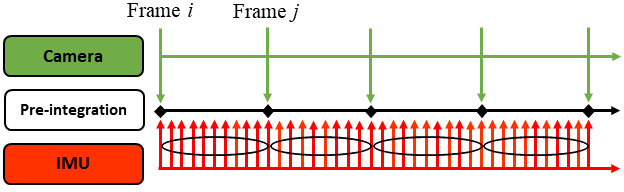
\includegraphics[width=1.0\linewidth]{Pictures/Preintegration/Introduction/Camera_IMU_example.jpg}
    \caption{Illustration of the sampling rate mismatch between an IMU and an exteroceptive sensor such as a camera or sonar. The IMU operates at hundreds of hertz, producing dense inertial measurements, while the sonar or camera generates new observations at a much lower rate. Preintegration combines all intermediate IMU readings into a single relative motion constraint that aligns with the moment a camera or sonar image is acquired.\textsuperscript{\cite{preintegration_camera_imu_picture}}}
    \label{fig:preintegration-camera-imu-example}
\end{figure}


